% \section*{Midterm 1 Review}

\renewcommand{\arraystretch}{1.25}

\subsection*{State-space models of systems}
In this unit, we are focusing on taking real-world systems and then working with them as matrix-vector equations. The first step to doing this is to represent systems with \textbf{state-space models}. \\
\newline
There are two parts to coming up with a state-space model:
\begin{enumerate}
    \item \textit{Choosing state variables.} These are the quantities that will appear in the $\vec{x}$ vector in an equation like 
    $$\frac{d}{dt}\vec{x}(t) = A\vec{x}(t) + B\vec{u}(t)$$ 
    \item \textit{Finding a differential or recurrence relation involving state variables:} i.e. find $\frac{d}{dt} \vec{x}$ in terms of $\vec{x}$ for a continuous-time system or find $\vec{x}(k + 1)$ in terms of $\vec{x}(k)$ for a discrete-time system. \\
    \newline
    Typically, this consists of filling in the elements of the $A$ matrix and $B$ vector, such as in the following equation:
    \begin{align*}
        \vec{x}(k + 1) = \begin{bmatrix}
            a_{11} & a_{12} \\
            a_{21} & a_{22}
        \end{bmatrix} \vec{x}(k) + \begin{bmatrix} b_1 \\ b_2 \end{bmatrix} u(t)
    \end{align*}
    However, \textbf{non-linear systems} cannot be represented as matrix-vector equations, so the state-space model can look as follows:
    \begin{align*}
        \frac{d}{dt} \vec{x}(t) = \begin{bmatrix}
            x_1^{\,2} + \cos(x_2) \\
            x_1^{\,3} - \sin(x_2)
        \end{bmatrix}
    \end{align*}
\end{enumerate}
For instance, when you analyzed the LRC circuit, you chose the voltage across the capacitor and the current through the inductor as your state variables and then used the current-voltage relationships of capacitors and inductors to come up with the following state-space representation:
\begin{align*}
    \frac{d}{dt} \begin{bmatrix} 
        I_L(t) \\ V_C(t)
    \end{bmatrix} = \begin{bmatrix}
        -R/L & -1/L \\
        1/C & 0
    \end{bmatrix} \begin{bmatrix} 
        I_L(t) \\ V_C(t)
    \end{bmatrix}
    \end{align*}

\subsection*{Linearization}
Many systems in the real world are nonlinear, which means that we cannot represent them with a matrix-vector equation. 
We would like to use linear tools (such as diagonalization) to solve these equations, so we typically linearize nonlinear systems. \\
\newline
\textbf{When is a system linear?} \\
\newline
A system is linear if it follows the \textbf{scaling} and \textbf{additivity} properties:
\begin{enumerate}
    \item \textbf{Scaling}: For a linear system $f$, $\boxed{f(ax) = af(x)}$ for every $a$ and for every $x$.
    \item \textbf{Additivity}: For a linear system $f$, $\boxed{f(x + y) = f(x) + f(y)}$ for every $x, y$.
\end{enumerate}
\textit{Note: Equations of the form $f(x) = ax + b$ with nonzero $b$ are not linear; they are considered to be \textbf{affine}}. \\
\newline
\textbf{Linearizing a nonlinear system} \\
\newline
We convert a nonlinear system into a linear system by using a first-order Taylor approximation:
$$\boxed{f(x) \approx f(x^*) + \frac{df}{dx} \bigg\rvert_{x = x^*} (x - x^*)}$$
Or, for an equation with an input, $u$:
$$\boxed{f(x, u) \approx f(x^*, u^*) + \frac{df}{dx} \bigg\rvert_{x = x^*} (x - x^*) + \frac{df}{du} \bigg\rvert_{u = u^*} (u - u^*)}$$
In these equations, we linearize the system around an \textbf{equilibrium point} or \textbf{operating point}, $(x^*, u^*)$. 
This is a point that we choose when making our approximation, typically so that
$$f(x^*, u^*) = 0$$
\newline
\textbf{Linearizing a system of nonlinear equations} \\
\newline
Say we have a system of nonlinear functions, typically represented by
\begin{align*}
    \vec{f}(\vec{x}) = \begin{bmatrix}
        f_1(x_1, \dots, x_n) \\
        \vdots \\
        f_m(x_1, \dots, x_n)
    \end{bmatrix}
\end{align*}
For these systems, you can linearize each equation using the partial derivative of the function with respect to each state variable:
\begin{center}
    \begin{align*}
        f_1(\vec{x}) \approx f_1(\vec{x}^*) + \frac{\partial f_1}{\partial x_1} \bigg\rvert_{x_1 = x_1^*} (x_1 - x_1^*) + \cdots + \frac{\partial f_1}{\partial x_n} \bigg\rvert_{x_n = x_n^*} (x_n - x_n^*) \\
        \vdots \\
        f_m(\vec{x}) \approx f_m(\vec{x}^*) + \frac{\partial f_m}{\partial x_1} \bigg\rvert_{x_1 = x_1^*} (x_1 - x_1^*) + \cdots + \frac{\partial f_m}{\partial x_n} \bigg\rvert_{x_n = x_n^*} (x_n - x_n^*)
    \end{align*}
\end{center}
In this case, we choose an $\vec{x}^*$ and $\vec{u}^*$ such that $\vec{f}(\vec{x}^*, \vec{u}^*) = \vec{0}$. \\
\newline
We can express this linearization as a matrix-vector equation:
\begin{align*}
    \vec{f}(\vec{x}) = \begin{bmatrix}
        \frac{\partial f_1}{\partial x_1} \bigg\rvert_{x_1^*} & \cdots & \frac{\partial f_1}{\partial x_n} \bigg\rvert_{x_n^*} \\
        \vdots & \ddots & \vdots \\
        \frac{\partial f_m}{\partial x_1} \bigg\rvert_{x_1^*} & \cdots & \frac{\partial f_m}{\partial x_n} \bigg\rvert_{x_n^*}
    \end{bmatrix} \begin{bmatrix}
        (x_1 - x_1^*) \\
        \vdots \\
        (x_n - x_n^*)
    \end{bmatrix} = \boxed{J_{\vec{x}} \vec{\delta x}}
\end{align*}
Where $J_{\vec{x}}$ is the \textbf{Jacobian matrix} of $\vec{f}$ with respect to $\vec{x}$ and $\vec{\delta x}$ is the distance of $\vec{x}$ from the equilibrium point. \\
\newline
If we are looking at a system of equations with a vector input, the linearization will be as follows
\begin{align*}
    \vec{f}(\vec{x}, \vec{u}) = \begin{bmatrix}
        \frac{\partial f_1}{\partial x_1} \bigg\rvert_{x_1^*} & \cdots & \frac{\partial f_1}{\partial x_n} \bigg\rvert_{x_n^*} \\
        \vdots & \ddots & \vdots \\
        \frac{\partial f_m}{\partial x_1} \bigg\rvert_{x_1^*} & \cdots & \frac{\partial f_m}{\partial x_n} \bigg\rvert_{x_n^*}
    \end{bmatrix} \begin{bmatrix}
        (x_1 - x_1^*) \\
        \vdots \\
        (x_n - x_n^*)
    \end{bmatrix} + \begin{bmatrix}
        \frac{\partial f_1}{\partial u_1} \bigg\rvert_{u_1^*} & \cdots & \frac{\partial f_1}{\partial u_k} \bigg\rvert_{u_k^*} \\
        \vdots & \ddots & \vdots \\
        \frac{\partial f_m}{\partial u_1} \bigg\rvert_{u_1^*} & \cdots & \frac{\partial f_m}{\partial u_k} \bigg\rvert_{u_k^*}
    \end{bmatrix} \begin{bmatrix}
        (u_1 - u_1^*) \\
        \vdots \\
        (u_k - u_k^*)
    \end{bmatrix} = \boxed{J_{\vec{x}} \vec{\delta x} + J_{\vec{u}} \vec{\delta u}}
\end{align*}


\subsection*{Stability}
A continuous- or discrete-time system is considered \textit{stable} if, for any bounded initial condition and series of inputs, the state remains bounded (if a quantity is \textit{bounded}, it is less than some finite constant at all times). We sometimes refer to this as \textbf{BIBO} (bounded input implies bounded output) \textbf{stability}. \\
\newline
For a system in \textit{discrete time}:
$$\vec{x}(k + 1) = A\vec{x}(k) + \vec{b}u(k)$$
The system is:
\begin{enumerate}
    \item \textbf{Stable}, if all eigenvalues have a \textbf{magnitude less than 1},
    \item \textbf{Unstable}, if at least one eigenvalue has a \textbf{magnitude greater than 1}, or
    \item \textbf{Marginally unstable}, if at least one eigenvalue has a magnitude of 1 and none have a magnitude greater than 1.
\end{enumerate}

For a system in \textit{continuous time}:
$$\frac{d}{dt} \vec{x}(t) = A\vec{x}(t) + \vec{b}u(t)$$
The system is:
\begin{enumerate}
    \item \textbf{Stable}, if all eigenvalues have a \textbf{negative real component},
    \item \textbf{Unstable}, if at least one eigenvalue has a \textbf{positive real component}, or
    \item \textbf{Marginally unstable}, if at least one eigenvalue has a real component of 0 and none have a positive real component.
\end{enumerate}

If we plot the eigenvalues on the \textit{complex plane}, a \textbf{discrete-time system} is stable if all eigenvalues are \textbf{strictly inside the unit circle} (left graph), and a \textbf{continuous-time system} is stable if all eigenvalues are on the left half of the plane (right graph): \\
\begin{tabular}{p{0.5\textwidth} p{0.5\textwidth}}
    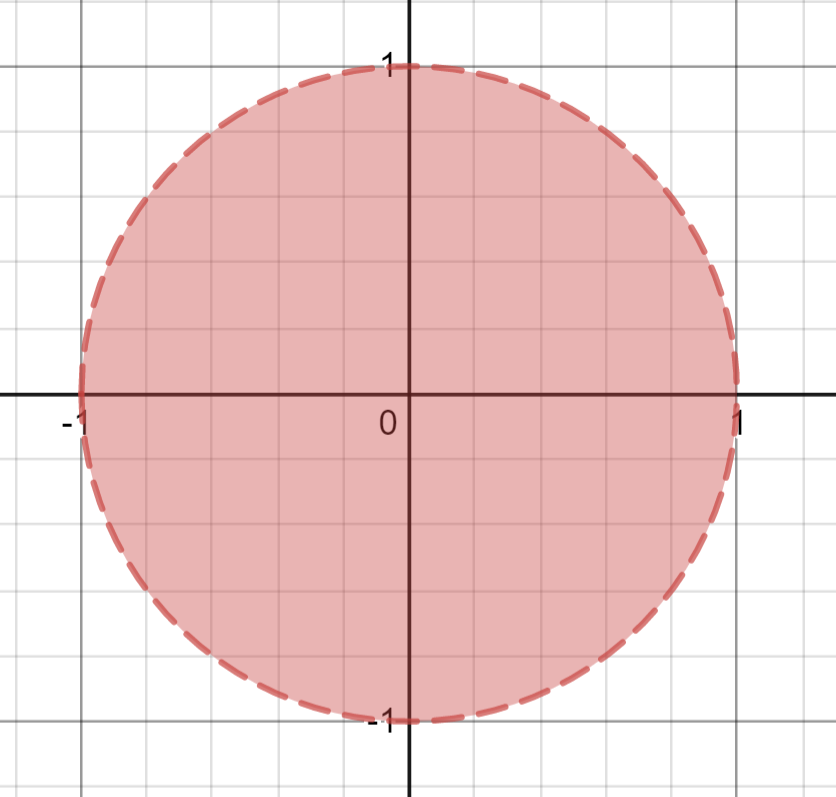
\includegraphics[width = 0.35 \textwidth]{\bank/../sp20/final/figures/discrete-stable.PNG} & 
    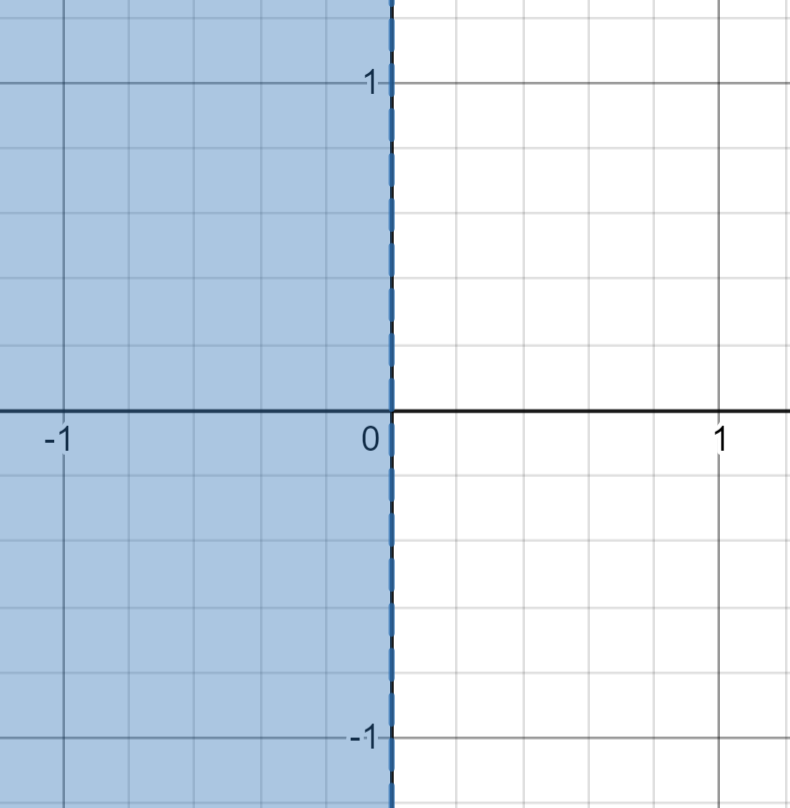
\includegraphics[width = 0.35 \textwidth]{\bank/../sp20/final/figures/continuous-stable.PNG}
\end{tabular}

An interesting case is \textit{upper-triangular matrices}. If a matrix is upper-triangular, its eigenvalues are on the diagonal, so to see if a system with an upper-triangular $A$ matrix is stable, you can look at its diagonal elements. \\
\newline

\textbf{Visualizing stability}: \\
We know that stable eigenvalues cause any input or initial condition to decay over time, unstable eigenvalues cause the state to grow exponentially, and marginally unstable eigenvalues cause any disturbance to neither decay nor grow. 
In addition, whether or not the eigenvalues have a complex component determines whether the state oscillates (continuous time), or rotates (discrete time). \\
\newline
The following plots will explore how complex eigenvalues affect the state evolution of stable and unstable systems.

\begin{tabular}{|m{0.3\textwidth}|m{0.3\textwidth}|m{0.4\textwidth}|}
    \multicolumn{3}{c}{Plots of $\vec{x}_1(k)$ for discrete-time systems with initial condition $\begin{bmatrix} 1 & 1 \end{bmatrix}^T$} \\
    \hline
    Real and Positive $\lambda$ & Complex or Negative $\lambda$ & Description \\
    \hline & & \\
    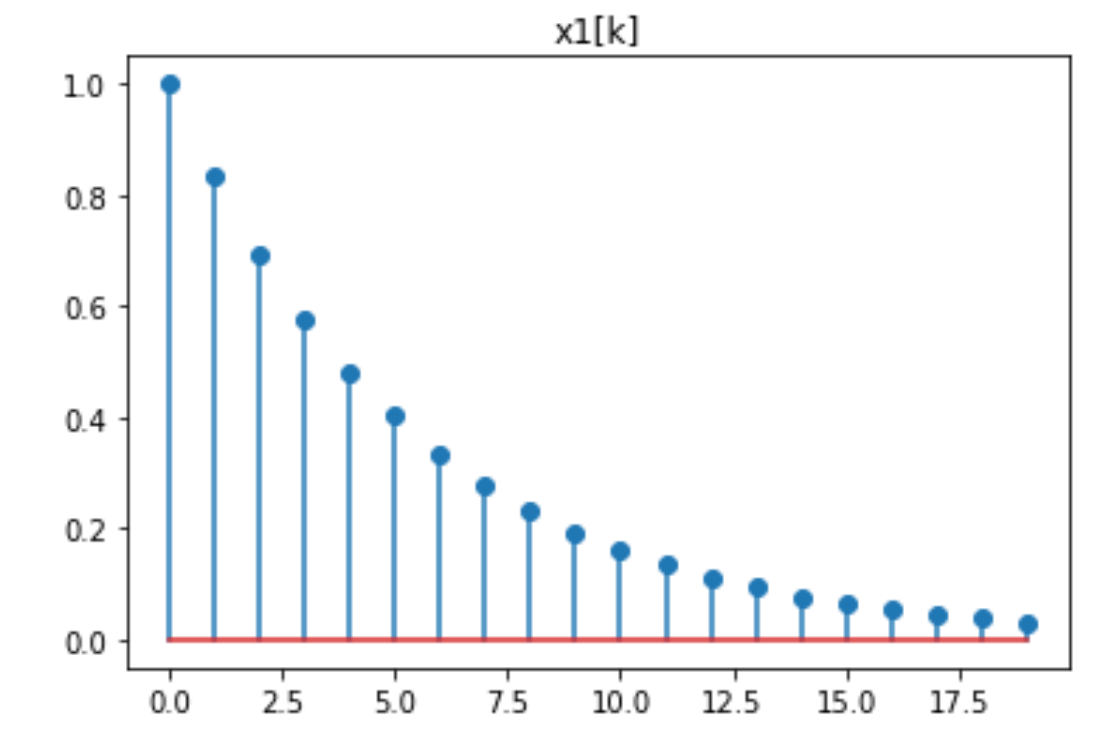
\includegraphics[width = 0.3 \textwidth]{\bank/stability/figures/discrete-graphs/stable-real-x1.PNG} &
    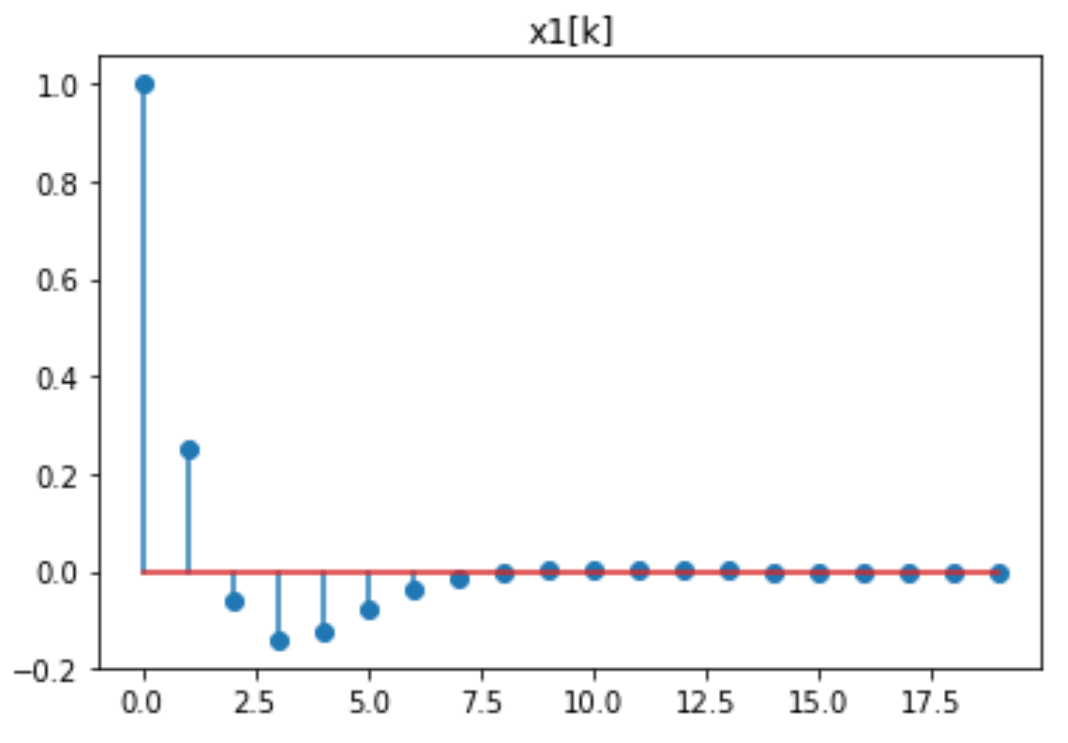
\includegraphics[width = 0.3 \textwidth]{\bank/stability/figures/discrete-graphs/stable-complex-x1.PNG} &
    \textbf{Stable system}: The system is stable, so the initial condition decays over time. When the eigenvalues are \textbf{real}, there is \textbf{no rotation}, but when they are \textbf{complex}, the state vector \textbf{rotates at every timestep}.\\
    \hline & & \\
    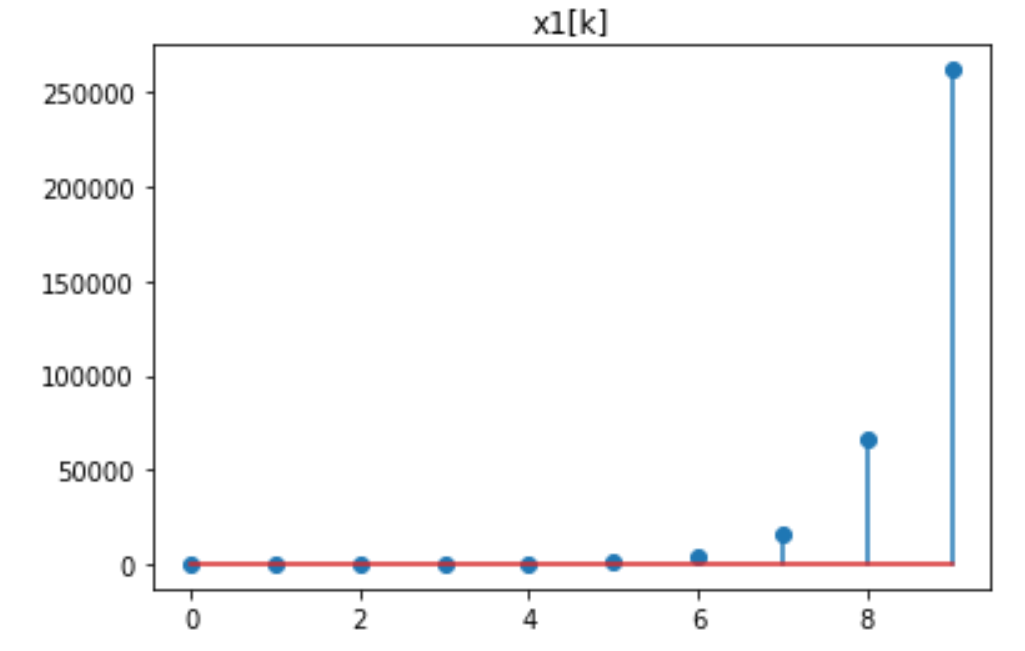
\includegraphics[width = 0.3 \textwidth]{\bank/stability/figures/discrete-graphs/unstable-real-x1.PNG} &
    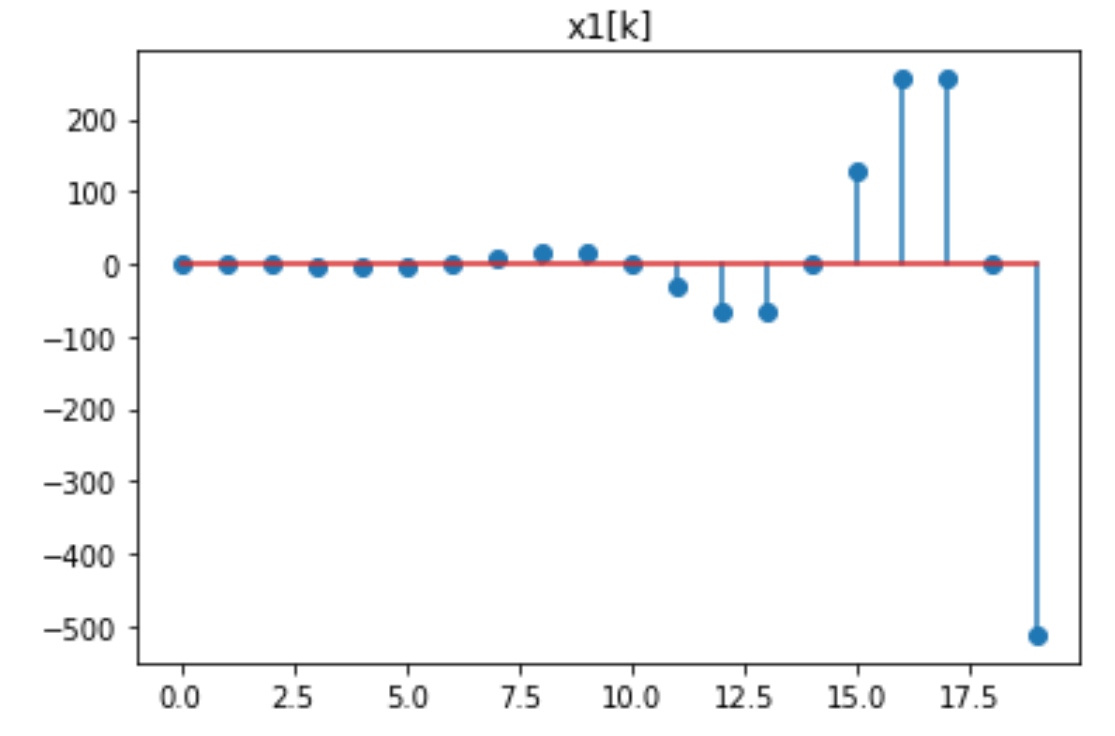
\includegraphics[width = 0.3 \textwidth]{\bank/stability/figures/discrete-graphs/unstable-complex-x1.PNG} &
    \textbf{Unstable system}: The system is unstable, so the initial condition grows exponentially. The state vector rotates only when the eigenvalues are complex. \\
    \hline & & \\
    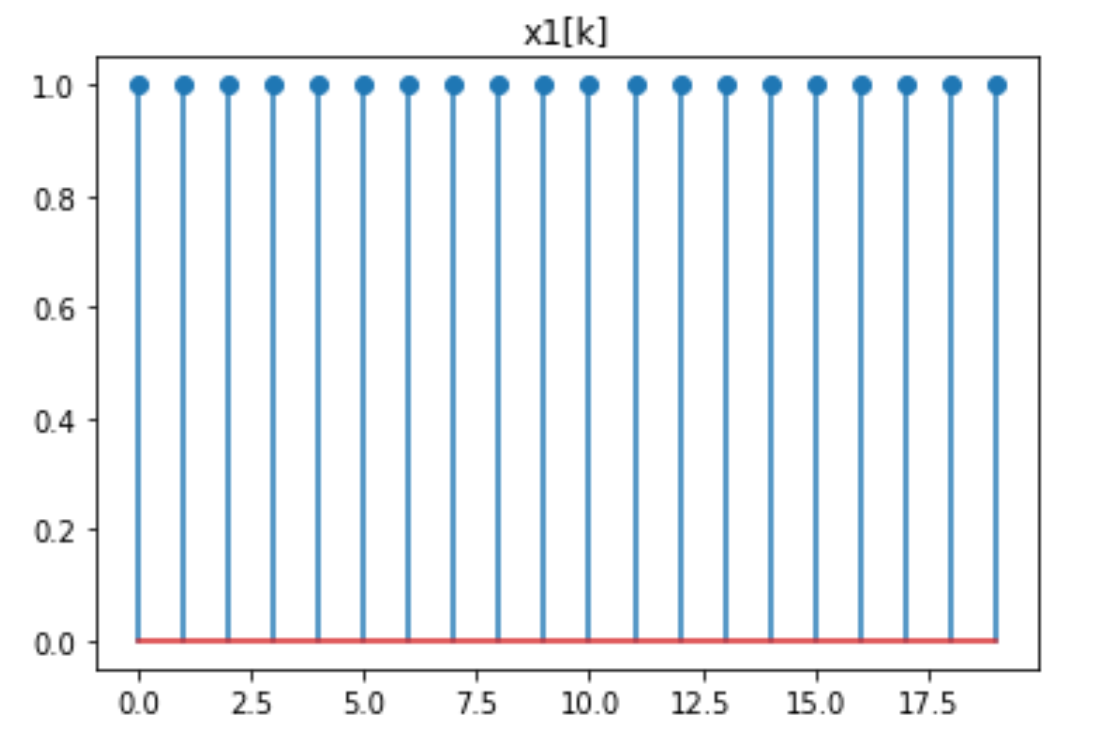
\includegraphics[width = 0.3 \textwidth]{\bank/stability/figures/discrete-graphs/marginal-real-x1.PNG} &
    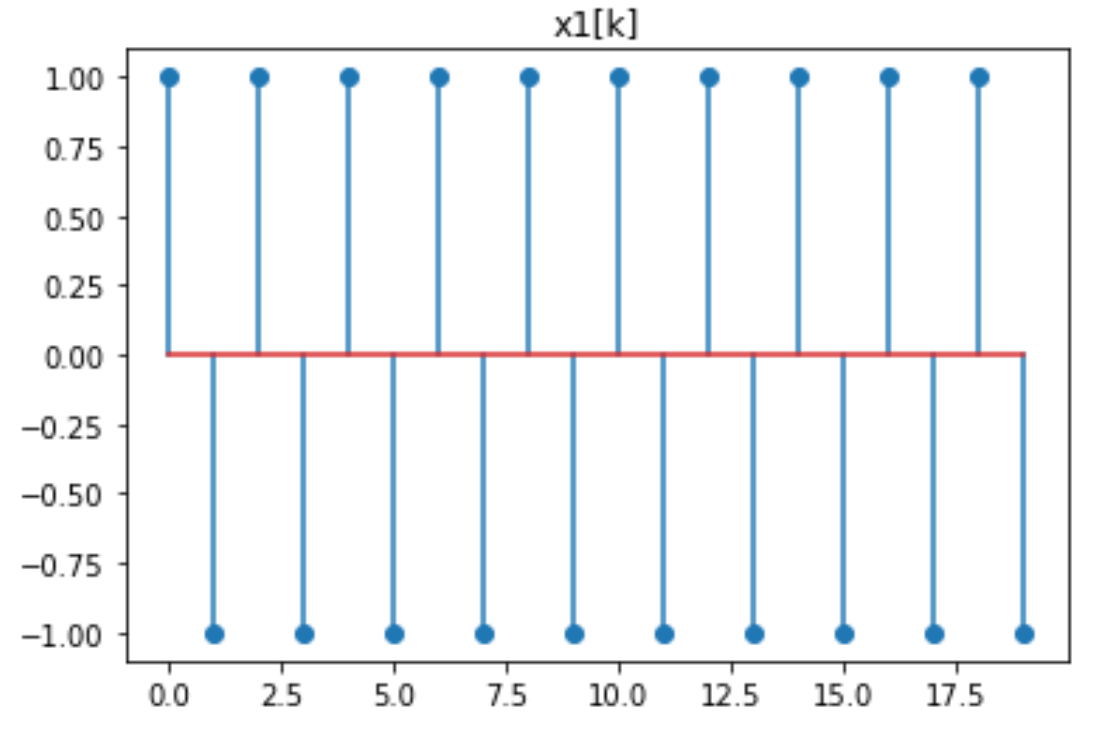
\includegraphics[width = 0.3 \textwidth]{\bank/stability/figures/discrete-graphs/marginal-negative-x1.PNG} &
    \textbf{Marginally unstable}: The initial condition neither grows nor decays. When both eigenvalues are 1, the state vector stays constant. When the eigenvalues are elsewhere on the unit circle, the state vector rotates.\vspace{2mm}\\
    \hline
\end{tabular}

\begin{tabular}{|m{0.3\textwidth}|m{0.3\textwidth}|m{0.4\textwidth}|}
     \multicolumn{3}{c}{Plots of $\vec{x}_1(t)$ for continuous-time systems with initial condition $\begin{bmatrix} 1 & 1 \end{bmatrix}^T$} \\
    \hline
    Real $\lambda$ & Complex or Imag. $\lambda$ & Description \\
    \hline & & \\
    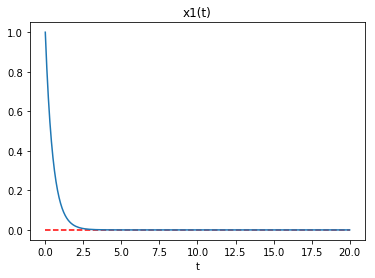
\includegraphics[width = 0.3 \textwidth]{\bank/stability/figures/continuous-graphs/real_negative_x1.png} &
    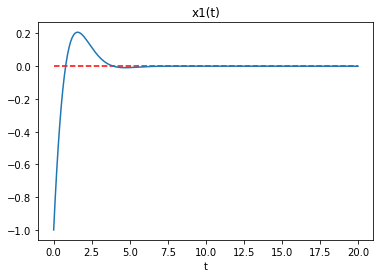
\includegraphics[width = 0.3 \textwidth]{\bank/stability/figures/continuous-graphs/complex_negative_x1.png} &
    \textbf{Stable system}: The system is stable, so the initial condition decays over time. When the eigenvalues are \textbf{real}, there is \textbf{no oscillation}, but when they are \textbf{complex}, the state \textbf{oscillates}. \vspace{2mm}\\
    \hline & & \\
    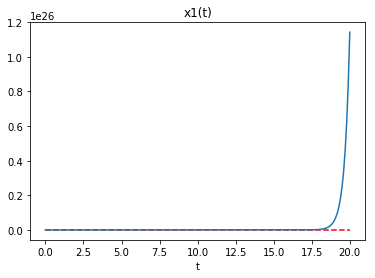
\includegraphics[width = 0.3 \textwidth]{\bank/stability/figures/continuous-graphs/real_positive_x1.png} &
    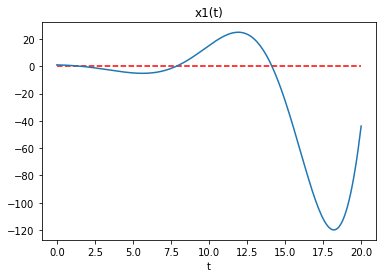
\includegraphics[width = 0.3 \textwidth]{\bank/stability/figures/continuous-graphs/complex_positive_x1.png} &
    \textbf{Unstable system}: The system is unstable, so the initial condition grows exponentially. The state oscillates only when the eigenvalues are complex. \\
    \hline & & \\
    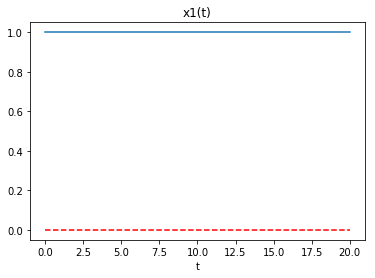
\includegraphics[width = 0.3 \textwidth]{\bank/stability/figures/continuous-graphs/zero_x1.png} &
    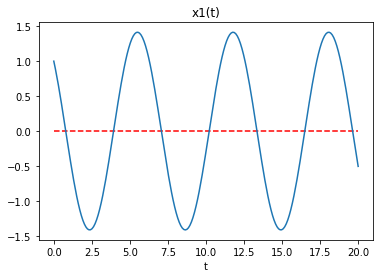
\includegraphics[width = 0.3 \textwidth]{\bank/stability/figures/continuous-graphs/imaginary_x1.png} &
    \textbf{Marginally unstable}: The initial condition neither grows nor decays. When both eigenvalues are 0, the state vector stays constant. When the eigenvalues are imaginary, the state oscillates without decaying.\\
    \hline
\end{tabular}

\subsection*{Controllability}
We say that a system of the form
$$\vec{x}(k + 1) = A\vec{x}(k) + \vec{b} u(k)$$
is controllable if, given any $\vec{x}(0)$, we can specify a series of control inputs $(u(0), u(1), \dots, u(n))$ to reach any state (so, $\vec{x}(n)$ can be anything we want it to be). \\
To determine whether a system is controllable, we define its controllability matrix to be
\begin{align*}
    \boxed{\mathcal{C} = \begin{bmatrix}
        \vec{b} & A\vec{b} & \cdots & A^{n - 1} \vec{b}
    \end{bmatrix}}
\end{align*}
Assuming we start at $\vec{x}(0) = \vec{0}$, we can reach any state in the span of the columns of $\mathcal{C}$, and therefore the system is controllable if the $\mathcal{C}$ is \textbf{full rank}, i.e., for an n-dimensional $\vec{x}$, the controllability matrix has n linearly independent columns. \\
\newline
\textbf{Controlling a system} \\
\newline
Assume we have a scalar input $u(k)$ and we want to see what states we can reach with $n$ controls if we start at $\vec{x}(0) = \vec{0}$. \\ 
\newline
Plugging the controls into the recurrence relation, we see that the first column of the controllability matrix corresponds to the last input ($u(n - 1)$), the second column corresponds to the second-to-last input ($u(n - 2)$), and the $n^{\text{th}}$ column corresponds to $u(0)$: 
\begin{align*}
    \vec{x}(n) = A\vec{x}(n - 1) + \vec{b} u(n - 1) \\
    \vec{x}(n) = A(A \vec{x}(n - 2) + \vec{b} u(n - 2)) + \vec{b} u(n - 1) \\
    = A^2 \vec{x}(n - 2) + A\vec{b} u(n - 2) + \vec{b} u(n - 1) \\
    \cdots
    \vec{x}(n) = A^n \vec{x}(0) + A^{n - 1} \vec{b} u(0) + \cdots +  A\vec{b} u(n - 2) + \vec{b} u(n - 1) \\
    = A^{n - 1} \vec{b} u(0) + \cdots +  A\vec{b} u(n - 2) + \vec{b} u(n - 1)
\end{align*}
So, if we want to pick control values such that a system reaches a certain $\vec{x}(n)$ starting at $\vec{x}(0) = \vec{0}$, we can use the relation
\begin{align*}
    \vec{x}(n) = \mathcal{C} \begin{bmatrix}
        u(n - 1) \\ \vdots \\ u(0)
    \end{bmatrix}
\end{align*}
and solve for your control inputs as follows:
\begin{align*}
    \begin{bmatrix}
        u(n - 1) \\ \vdots \\ u(0)
    \end{bmatrix} = \boxed{\mathcal{C}^{-1} \vec{x}(n)}
\end{align*}


\subsection*{Feedback Control and Eigenvalue Placement}
Consider a system that is controllable but has unstable eigenvalues:
\begin{align*}
    \vec{x}(k + 1) = A\vec{x}(k) + \vec{b}u(k)
\end{align*}
We can use the fact that the system is controllable to place its eigenvalues wherever we want by applying a \textit{feedback control}, where the control input depends on the current state. Depending on the problem, the feedback input will either be of the form $u(t) = \vec{f^T} \vec{x}(k)$ or $u(t) = -\vec{f^T} \vec{x}(k)$. We will use the first one in this worksheet, but you should expect to see both forms.
\begin{align*}
    \vec{x}(k + 1) = A\vec{x}(k) + \vec{b}\vec{f}^T \vec{x}(k)
\end{align*}
We can rewrite this system as follows:
\begin{align*}
    \vec{x}(k + 1) = (A + \vec{b}\vec{f}^T) \vec{x}(k)
\end{align*}
The new state transition matrix for the system is $(A + \vec{b}\vec{f}^T)$. Because the system is controllable, we can pick the elements of the feedback coefficient vector $\vec{f}$ to place the eigenvalues of our system wherever we choose. \\
\newline

\subsection*{System Identification}
If we don't know the parameters of our system (i.e. the $A$ matrix and $\vec{b}$ vector) but we do have a series of inputs and outputs to the system, we can use least squares to solve for the elements of $A$ and $\vec{b}$. \\
\newline
First, let us consider a 2-dimensional system with a scalar input.
\begin{align*}
    \begin{bmatrix}
        x_1(k + 1) \\ x_2(k + 1)
    \end{bmatrix} = \begin{bmatrix}
        a_{11} & a_{12} \\
        a_{21} & a_{22}
    \end{bmatrix} \begin{bmatrix}
        x_1(k) \\ x_2(k)
    \end{bmatrix} + \begin{bmatrix}
        b_1 \\ b_2
    \end{bmatrix} u(k)
\end{align*}
Also, let's say we are given the following data points: $\vec{x}(0), \dots, \vec{x}(m)$ and $u(0), \dots, u(m - 1)$. \\
\newline
In order to perform system identification, we want to format the system as a least squares problem:
\begin{align*}
    D\vec{p} \approx \vec{y}
\end{align*}
$\vec{p}$ is our vector of unknowns, so we populate it with the elements of $A$ and $\vec{b}$:
\begin{align*}
    \vec{p} = \begin{bmatrix}
        a_{11} & a_{12} & a_{21} & a_{22} & b_1 & b_2
    \end{bmatrix}^T
\end{align*}
We can view $\vec{y}$ as the output of the system, so we can populate with $\vec{x}(1), \dots, \vec{x}(m)$
\begin{align*}
    \vec{y} = \begin{bmatrix}
        x_1(1) & x_2(1) & \cdots & x_1(m) & x_2(m)
    \end{bmatrix}^T
\end{align*}
Now, we need to find the elements of the $D$ matrix to complete the relationship between $\vec{p}$ and $\vec{y}$. 
From the matrix-vector representation of the system, we get scalar equations of the form
\begin{align*}
    x_1(k + 1) = a_{11} x_1(k) + a_{12} x_2(k) + b_1 u(k) \\
    x_2(k + 1) = a_{21} x_1(k) + a_{22} x_2(k) + b_2 u(k) 
\end{align*}
So, we have the following least-squares problem:
\begin{align*}
    \begin{bmatrix}
        x_1(1) \\ x_2(1) \\ x_1(2) \\ x_2(2) \cdots \\ x_1(m) \\ x_2(m)
    \end{bmatrix} = \begin{bmatrix}
        x_1(0) & x_2(0) & 0 & 0 & u(0) & 0 \\
        0 & 0 & x_1(0) & x_2(0) & 0 & u(0) \\
        x_1(1) & x_2(1) & 0 & 0 & u(1) & 0 \\
        0 & 0 & x_1(1) & x_2(1) & 0 & u(1) \\
        \vdots & \vdots & \vdots & \vdots & \vdots & \vdots \\
        x_1(m - 1) & x_2(m - 1) & 0 & 0 & u(m - 1) & 0 \\
        0 & 0 & x_1(m - 1) & x_2(m - 1) & 0 & u(m - 1)
    \end{bmatrix} \begin{bmatrix}
        a_{11} \\ a_{12} \\ a_{21} \\ a_{22} \\ b_1 \\ b_2
    \end{bmatrix}
\end{align*}
From here, we can solve for $\vec{p}$ using the least-squares formula:
$$\boxed{\vec{p} = (D^T D)^{-1} D^T \vec{y}}$$
This also extrapolates to systems of higher dimension.
\newline
\textit{Note: At the very least, you need $\vec{x}(0), \dots \vec{x(3)}$ and $u(0), u(1), u(2)$ because we have 6 unknowns and need 6 equations to have a unique solution.}

\subsection*{SVD}
Now, we will look at \textbf{singular value decomposition}, which decomposes any arbitrary matrix into two orthonormal matrices and a diagonal matrix:
\begin{align*}
    \boxed{A = U \Sigma V^T} 
\end{align*}
Where the columns of $U$ are orthonormal, the rows of $V^T$ are orthonormal, and $\Sigma$ has the \textbf{singular values} of the system on the diagonal and is zero elsewhere. \\
\newline
The SVD can also be written in \textbf{outer product form} as follows:
\begin{align*}
    \boxed{A = \sum \sigma_i \vec{u}_i \vec{v}^T_i}
\end{align*}
$\vec{u}_i \vec{v}^T_i$ is the outer product of $\vec{u}$ and $\vec{v}$, which results in a rank-one matrix. So, if $A$ is a rank-k matrix, $A$ can be expressed as the sum of $k$ rank-one matrices, each scaled by the corresponding singular value. \\
\newline
This is useful in approximating high-rank matrices with lower-rank ones. If we want to approximate $A$ as a rank-j matrix where $j < k$, we can take the first $j$ terms of the outer-product form of the SVD (the terms that correspond to the $j$ largest singular values):
\begin{align*}
    \boxed{A \approx \sum_{i = 1}^{j} \sigma_i \vec{u}_i \vec{v}^T_i}
\end{align*}
\newline
\textbf{Elements of the SVD}
\begin{enumerate}
    \item The columns of $U$ are orthonormal eigenvectors of the matrix $AA^T$.
    \item The columns of $V$ (rows of $V^T$) are orthonormal eigenvectors of the matrix $A^T A$.
    \item The diagonal elements of $\Sigma$ are the singular values of $A$. The $i^{\text{th}}$ singular value, $\sigma_i = \sqrt{\lambda_i}$, where $\lambda_i$ is the $i^{\text{th}}$ eigenvalue of $A^T A$ and $A A^T$ (it can be proven that both have the same eigenvalues! See the SVD intuition section for why that is the case.) \\
    \textit{Note: all singular values are real and nonnegative.}
\end{enumerate}

\textbf{Compact SVD} \\
\newline
For the compact SVD, we only look at the nonzero eigenvalues of $A^T A$ and $AA^T$ (we don't include eigenvectors in the nullspaces of $A^T A$ and $A A^T$). \\
\newline
Let's say $A$ is an $n \times m$ matrix of rank $k$ (has k linearly independent columns). Then, there are $k$ nonzero singular values, as well as k columns in the $U$ and $V$ matrices. So, \textbf{$U$ is $n \times k$}, \textbf{$\Sigma$ is $k \times k$}, and \textbf{$V^T$ is $k \times m$} \\
\newline
\textbf{Computing the Compact SVD}
\begin{enumerate}
    \item Find the eigenvalues and nonzero eigenvectors of either $A A^T$ (to compute $U$) or $A^T A$ (to compute $V$). You can start with either, but it is easier to start with the matrix that has smaller dimensions, i.e. $A^T A$ for tall matrices and $AA^T$ for wide matrices. 
    \item Order the eigenvalues from largest to smallest, including repeated eigenvalues. The square root of the $i^{\text{th}}$ eigenvalue is $\sigma_i$. If you started out with $AA^T$, the eigenvector corresponding to $\lambda_i$ is the $i^{\text{th}}$ column of the $U$ matrix ($\vec{u}_i$). Otherwise, it is the $i^{\text{\th}}$ column of the $V$ matrix.
    \item If you started out with $AA^T$, compute $\vec{v}_i$ as $\frac{A^T \vec{u}_i}{\sigma_i}$. Otherwise, compute $\vec{u}$ as $\frac{A \vec{v}_i}{\sigma_i}$.
\end{enumerate}

\textbf{Full SVD} \\
\newline
For the full SVD, we start with the compact SVD and then add eigenvectors in the nullspace of $AA^T$ to $U$ and eigenvectors in the nullspace of $A^TA$ to $V$. \\
\newline
Let's say $A$ is an $n \times m$ matrix of rank $k$. Then, for the full SVD, $U$ will be an orthonormal $n \times n$ matrix, $\Sigma$ will have the dimensions $n \times m$ (same as the original A matrix), and $V$ will be an orthonormal $m \times m$ matrix. \\
\newline
\textbf{Computing the Full SVD}
\begin{enumerate}
    \item Compute the compact SVD.
    \item Now, let's fill in $\vec{u}_{k+1}, \dots, \vec{u}_n$. We have found the eigenvectors of $AA^T$ with nonzero eigenvalues, so now we compute the eigenspace for $\lambda = 0$. To do so, find an orthonormal basis for the nullspace of $AA^T$ and append it to your $U$ matrix.
    \item Then, do the same for $V$. Find an orthonormal basis for the nullspace of $A^T A$ and append it to your $V$ matrix.
    \item Finally, we need to modify $\Sigma$ so that it is $n \times m$ (so the matrix multiplication in $U \Sigma V^T$ works out). Zero-pad $\Sigma$ until it has dimensions $n \times m$.
\end{enumerate}
\textit{Side note (out-of-scope intuition): $U$ is guaranteed to be orthogonal because the set of vectors $\{\vec{u}_{k + 1}, \dots, \vec{u}_n\}$ is orthogonal to $\{\vec{u}_1, \dots, \vec{u}_k$\}. 
This is because $\vec{u}_1, \dots, \vec{u}_k$ come from the columnspace of $A$ and $\vec{u}_{k + 1}, \dots, \vec{u}_n$ come from the nullspace of $A^T$, which are orthogonal subspaces. 
Similar logic can be applied to $V$ if we switch $A$ and $A^T$.} \\
\newline
\textbf{SVD Intuition (Compact SVD)} \\
\newline
The \textbf{Spectral Theorem} states that symmetric matrices in $\mathbb{R}^{n\times n}$ have $n$ \textbf{orthogonal eigenvectors}, and all eigenvalues are \textbf{real}. In addition, for the symmetric matrices $A^T A$ and $AA^T$, it can be proven that all eigenvalues are \textbf{nonnegative}. \\
\newline
For the SVD, we consider the symmetric matrices $AA^T$ and $A^T A$. We want to show that
$$AV = U\Sigma$$
where $U$ and $V$ are both orthonormal because they consist of eigenvalues of a symmetric matrix.
\begin{enumerate}
    \item If $\vec{v}$ is an eigenvalue of $A^T A$ with eigenvalue $\lambda$, then $A\vec{v}$ is an eigenvalue of $AA^T$ with the same eigenvalue:
    $$A^T A \vec{v} = \lambda \vec{v}$$
    Left-multiply both sides by $A$ to get
    $$A A^T (A \vec{v}) = \lambda (A \vec{v})$$
    \item We want to choose orthonormal eigenvectors for $AA^T$ and $A^T A$. 
    So, if we choose $\vec{v}$ to have norm 1, we want to find an eigenvector $\vec{u}$ of $AA^T$ that also has norm 1. 
    The norm of $A \vec{v}$ is $\lambda$:
    $$||A\vec{v}|| = \sqrt{\vec{v}^T A^T A \vec{v}} = \sqrt{\lambda ||\vec{v}||} = \sqrt{\lambda}$$
    So, we define $\vec{u}$ to be
    $$\vec{u} = \frac{A \vec{v}}{\sqrt{\lambda}} = \frac{A \vec{v}}{\sigma}$$
    \item Knowing that 
    $$\sigma \vec{u} = A \vec{v}$$
    If we define $U$ and $V$ as
    \begin{align*}
        U = \begin{bmatrix} \vec{u}_1 & \cdots & \vec{u}_k \end{bmatrix} \\
        V = \begin{bmatrix} \vec{v}_1 & \cdots & \vec{v}_k \end{bmatrix}
    \end{align*}
    Then the equation relating $U$ and $V$ can be written as
    $$U\Sigma = AV$$
    \item From there, we can right-multiply both sides by the transpose of $V$. 
    $$AVV^T = U \Sigma V^T$$
    $VV^T$ is not quite the identity matrix (it would be if $V$ was square, since $V$ is orthonormal), but it can be proven that $AVV^T = A$ (look at note 9B for more information). So,
    $$A = U \Sigma V^T$$
\end{enumerate}